\documentclass[12pt]{beamer}
\usetheme{Boadilla}
\usepackage{booktabs}
\usepackage{tikz}
\usepackage{pgfplots}
\renewcommand{\arraystretch}{1.25}
\usetikzlibrary{trees}
\title[ECON2843]{Lecture 4}
\subtitle{Part 2 Probability and Distributions}
\date{}
\usepackage{amsmath,amssymb,mathtools,wasysym}
\begin{document}
	\begin{frame}
		\titlepage
	\end{frame}
\begin{frame}
Let's start from something about gambling...
\end{frame}
\begin{frame}
	A casino offer you a game of chance: a fair coin is tossed at every stage.
	\begin{itemize}
		\item[$\blacktriangleright$] The initial stake begins at \$2 and is {\sl doubled} every time tails appears.
		\item[$\blacktriangleright$] The first time heads appears, the game ends and the player wins whatever is the current stake.
		\item[$\blacktriangleright$] Thus the player wins \$2 if heads appears on the first toss, \$4 if tails appears on the first toss and heads on the second, \$8 if tails appears on the first two tosses and heads on the third, and so on.
	\end{itemize}
	Question: How much are you willing to pay for playing this game?
\end{frame}
\begin{frame}{St. Petersburg paradox}
Your expected return for playing this game:
\begin{align*}
	\text{Expected Return}&=2\times\frac{1}{2}+4\times\frac{1}{4}+8\times\frac{1}{8}+\cdots\\
	&=2\times\frac{1}{2}+2^2\times\frac{1}{2^2}+2^3\times\frac{1}{2^3}+\cdots\\
	&= \sum_{n=1}^{\infty} 2^n \cdot \frac{1}{2^n}= \sum_{n=1}^{\infty} 1= \infty
\end{align*}

Question: Are you willing to pay an infinite number for this game?

Let me ask you again, how much are you willing to pay?
\end{frame}
\begin{frame}{Random Experiment}
	\begin{itemize}
		\item[$\blacktriangleright$] A {\bf random experiment} is a process that results in one of several possible outcomes, none of which can be predicted with certainty.
		
		For example:
		\begin{itemize}
			\item Rolling a conventional die. Possible outcomes are 1, 2, 3, 4, 5 or 6.
			\item Flipping a coin. Possible outcomes are heads or tails.
     	\end{itemize}
		\item[$\blacktriangleright$] Outcomes are denoted by $O_i$.
	\end{itemize}
\end{frame}
\begin{frame}{Sample Space}
	\begin{itemize}
		\item[$\blacktriangleright$] The sample space of a random experiment is a list of all the possible outcomes and is denoted by
		$$S=\{O_1,O_2,O_3,\cdots\}$$
		For example, when flipping a coin, $S=\{H,T\}$
		\item[$\blacktriangleright$] The outcomes in a sample space must be both {\sl mutually exclusive} and {\sl exhaustive}.
		\begin{itemize}
			\item {\bf Mutually exclusive}: No two outcomes can both occur at the same time on any single trial of the experiment.
			\item {\bf Exhaustive}: The sample space must include all possible outcomes that can occur.
		\end{itemize}
	\end{itemize}
\end{frame}
\begin{frame}{Probabilities of Outcomes}
	\begin{itemize}
		\item[$\blacktriangleright$] The probability of an outcome occurring on a single trial is written as $P(O_i)$.
		\item[$\blacktriangleright$] Probabilities associated with the outcomes in a sample space must satisfy two important requirements:
		\begin{itemize}
			\item $0\le P(O_i)\le1$ for all $i$.
			\item $\sum_iP(O_i)=1$.
		\end{itemize}
	\end{itemize}
\end{frame}
\begin{frame}{Classical Approach}
	The {\sl classical approach} is based on the assumption that the outcomes of an experiment are equally likely to happen.
	\begin{itemize}
		\item[$\blacktriangleright$] Suppose we roll a {\color{red}fair} six-sided dice.
		\item[$\blacktriangleright$] What is the probability of rolling a 5?
		\item[$\blacktriangleright$] The sample space is $S=\{1,2,3,4,5,6\}$.
		\item[$\blacktriangleright$] Assuming all six outcomes are equally likely, the probability of rolling a 5 is $P(5)=\frac{1}{6}$.
		\item[$\blacktriangleright$] Note that in more complicated experiments, we often need to use mathematical rules to count the total number of outcomes.
	\end{itemize}
\end{frame}
\begin{frame}{Relative Frequency Approach}
	The relative frequency approach defines probability as the long-run relative frequency with which an outcomes occurs.
	\begin{itemize}
		\item[$\blacktriangleright$] Suppose we roll a {\color{red}loaded} six-sided dice.
		
		For example:
	\end{itemize}
\begin{figure}[htbp]
	\centering
	\begin{minipage}{0.4\textwidth}
		\centering
		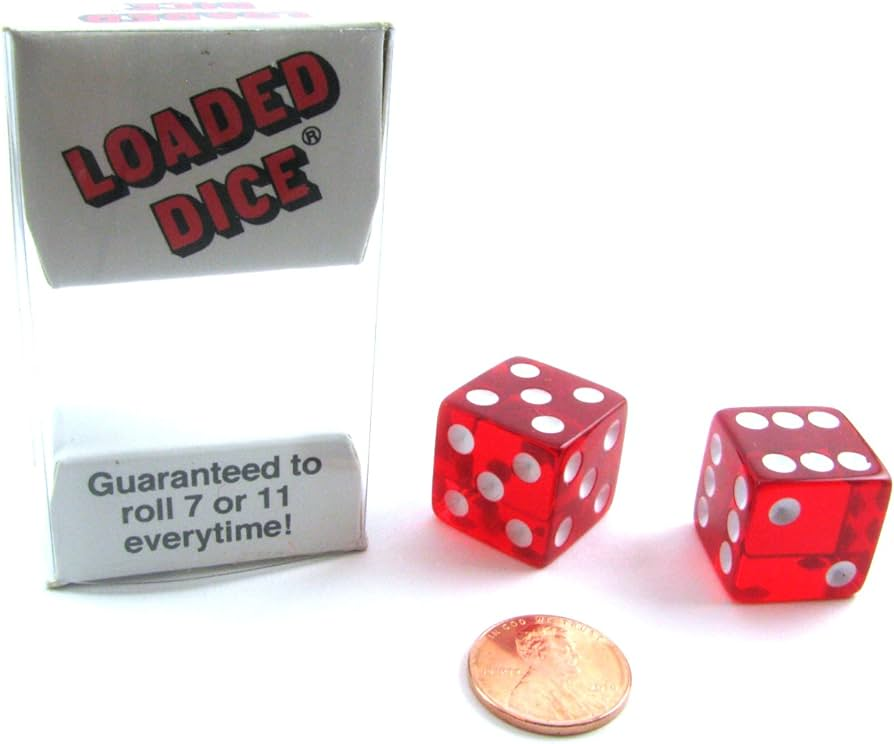
\includegraphics[width=\textwidth]{dice.jpg}
	\end{minipage}\hfill
	\begin{minipage}{0.45\textwidth}
		\centering
		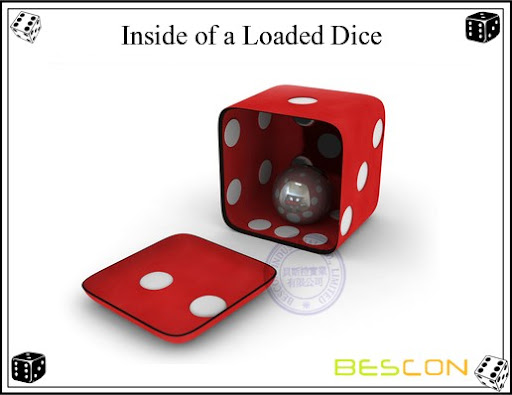
\includegraphics[width=\textwidth]{loaded2.jpg}
	\end{minipage}
\end{figure}
\end{frame}
\begin{frame}{Relative Frequency Approach}
	The {\sl relative frequency approach} defines probability as the long-run relative frequency with which an outcomes occurs.
	\begin{itemize}
		\item[$\blacktriangleright$] Suppose we roll a {\color{red}loaded} six-sided dice.
		\item[$\blacktriangleright$] What is the probability of rolling a 5?
		\item[$\blacktriangleright$] We can't assume equally likely outcomes.
		\item[$\blacktriangleright$] But suppose we know that in the past 1000 rolls, a 5 came up 190 times.
		\item[$\blacktriangleright$] Based on this past history, we assign the probability of rolling a 5 to be the long-run relative frequency, i.e., $\frac{19}{100}=0.19$.
	\end{itemize}
\end{frame}
\begin{frame}{Subjective Approach}
	The {\sl subjective approach} is based on personal judgment, accumulation of knowledge, and experience.
	\begin{itemize}
		\item[$\blacktriangleright$] Suppose we roll a {\color{red}loaded} six-sided dice.
		\item[$\blacktriangleright$] What is the probability of rolling a 5?
		\item[$\blacktriangleright$] We can't assume equally likely outcomes.
		\item[$\blacktriangleright$] Suppose I have no historical data on the die.
		\item[$\blacktriangleright$] So, based on what I read about loaded dice on Wikipedia and also based on how this particular die feels in my hand (weight distribution, size, etc.), I decide that the probability of rolling a 5 is 0.2.
	\end{itemize}
\end{frame}
\begin{frame}{Events}
	\begin{itemize}
		\item[$\blacktriangleright$] A simple event is an individual outcome from the sample space.
		\item[$\blacktriangleright$] An event is a collection of one or more simple events (or outcomes).
	\end{itemize}
For example, when rolling a die, let $A$ denote the event that an odd number comes up. Then $A=\{1,3,5\}$.
\end{frame}
\begin{frame}{Probability of an Event}
	\begin{itemize}
		\item[$\blacktriangleright$] The probability of an event is equal to the sum of the probabilities of the simple events that make up the event:
		$$P(A)=P(1)+P(3)+P(5)=\frac{1}{6}+\frac{1}{6}+\frac{1}{6}=\frac{1}{2}$$
		\item[$\blacktriangleright$] If we assume all simple events have equal probability, we can also determine the probability of an event by counting the number of simple events that make up the event:
		$$P(A)=\frac{\text{number of simple events in }A}{\text{number of simple events in }S}=\frac{3}{6}=\frac{1}{2}$$
	\end{itemize}
\end{frame}
\begin{frame}{Combining Events}
	\begin{itemize}
		\item[$\blacktriangleright$] There are some important ways in which events cane combined that we will encounter repeatedly throughout this course.
		\item[$\blacktriangleright$] Suppose we have two events, $A$ and $B$.
		\begin{itemize}
			\item For example, suppose we roll a conventional die and let $A = \{1, 3, 5\}$ denote the event of rolling an odd number and let $B = \{3,4\}$ denote the event of rolling either a 3 or a 4.
		\end{itemize}
	\end{itemize}
\end{frame}
\begin{frame}{Venn Diagrams}
	\begin{itemize}
		\item[$\blacktriangleright$] We can use Venn diagrams to visually describe the events.
	\end{itemize}
	\centering
	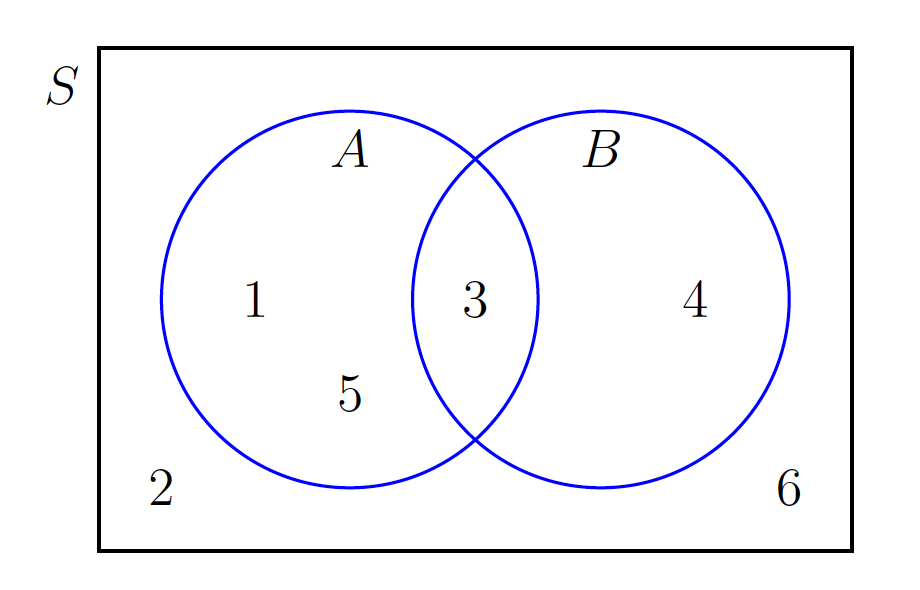
\includegraphics[width=8cm]{venn.png}
\end{frame}
\begin{frame}{Intersection}
	\begin{itemize}
		\item[$\blacktriangleright$] The {\bf intersection} of $A$ and $B$, denoted by $A\cap B$, is the event that happens when both $A$ and $B$ occur.
		\begin{itemize}
			\item For example, $A\cap B=\{3\}$.
		\end{itemize}
	\end{itemize}
	\centering
	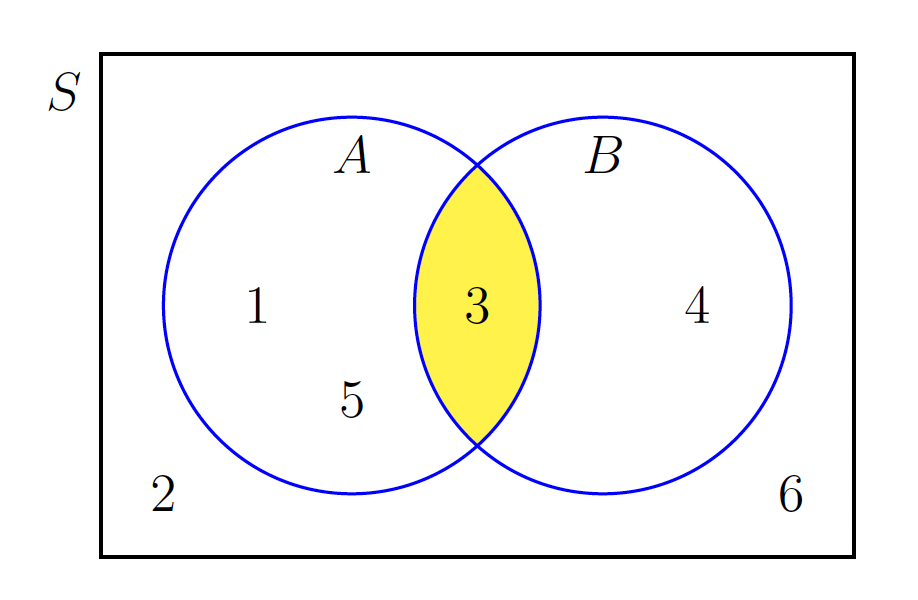
\includegraphics[width=8cm]{venn2.png}
\end{frame}
\begin{frame}{Union}
	\begin{itemize}
		\item[$\blacktriangleright$] The {\bf union} of $A$ and $B$, denoted by $A\cup B$, is the event that happens when either $A$ and $B$ occur.
		\begin{itemize}
			\item For example, $A\cup B=\{1,3,4,5\}$.
		\end{itemize}
	\end{itemize}
	\centering
	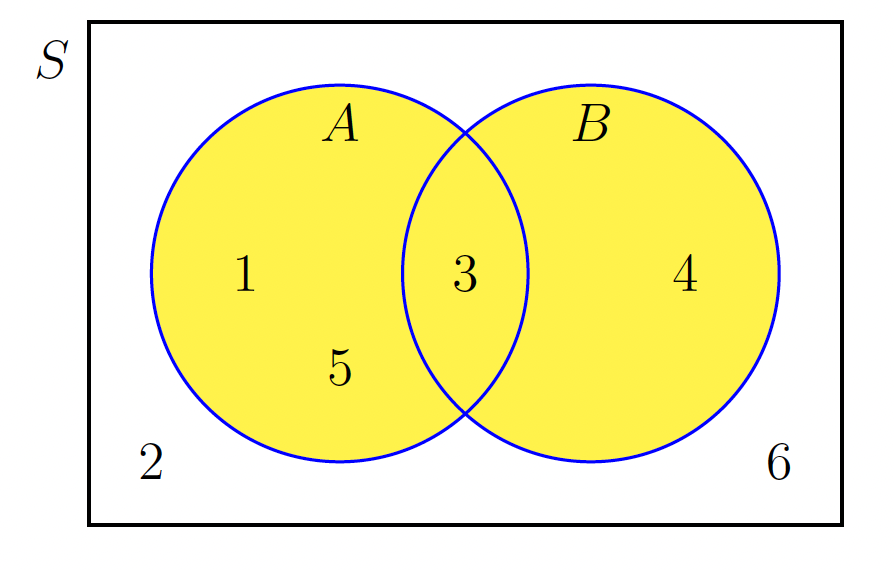
\includegraphics[width=8cm]{venn3.png}
\end{frame}
\begin{frame}{Complement}
	\begin{itemize}
		\item[$\blacktriangleright$] The {\bf complement} of $A$, denoted $A^C$, is the event that happens when $A$ does not occur.
		\begin{itemize}
			\item For example, $A^C=\{2,4,6\}$.
		\end{itemize}
	\end{itemize}
	\centering
	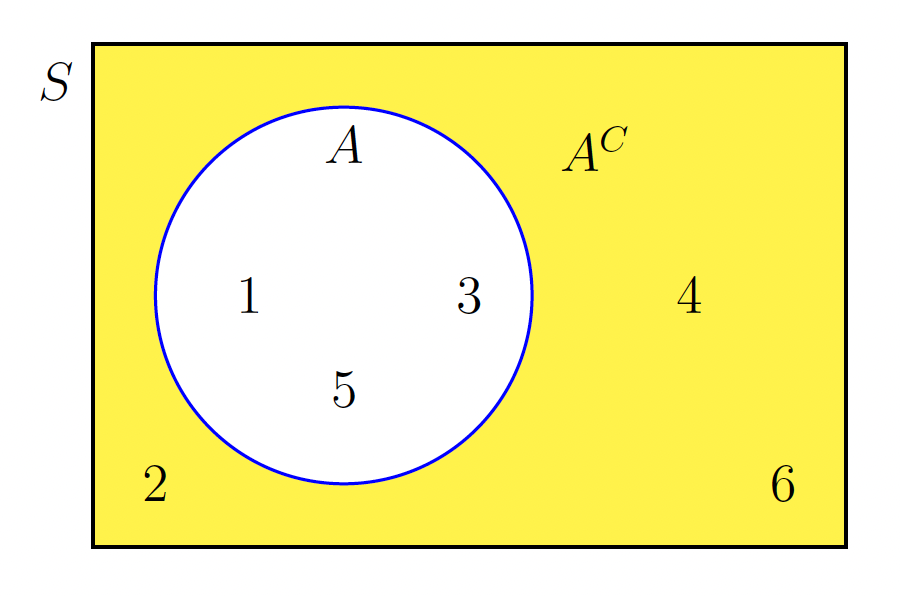
\includegraphics[width=8cm]{venn4.png}
\end{frame}
\begin{frame}{Intersection and Union}
	\begin{itemize}
		\item[$\blacktriangleright$] Both intersection and union are commutative operators.
		\item[$\blacktriangleright$] That is, for any events $A$ and $B$, the following are true:
$$A\cap B=B\cap A$$ and $$A\cup B=B\cup A$$
\item[$\blacktriangleright$]The order of the events does not matter.
	\end{itemize}
\end{frame}
\begin{frame}{Important Facts}
	\begin{itemize}
		\item[$\blacktriangleright$] For the sample space $S$,
		$$P(S)=1$$
		\item[$\blacktriangleright$] For any event $A$,
		$$0\le P(A)\le1$$
		\item[$\blacktriangleright$]If $A$ and $B$ are mutually exclusive (i.e., $A\cap B=\emptyset$), then $$P(A\cap B)=0$$
	\end{itemize}
\end{frame}
\begin{frame}{Joint Probability}
	\begin{itemize}
		\item[$\blacktriangleright$] A joint probability is the probability of the intersection of two or more events.
		\begin{itemize}
			\item For example, $P(A\cap B)$ or $P(A\cap B\cap C)$.
		\end{itemize}
		\item[$\blacktriangleright$] Suppose we are investigating the relationship between how well a mutual fund performs and where the fund manager earned their MBA.
	\end{itemize}
\end{frame}
\begin{frame}{Joint Probability}
	Let's define the following events:
	\begin{itemize}
		\item[$\blacktriangleright$] Let event $A_1$ be the event that the fund manager graduated from a program ranked in the top 10.
		\item[$\blacktriangleright$] Let $A_2$ be the event that the fund manager graduated from a program ranked between 10 and 20.
		\item[$\blacktriangleright$] Let $A_3$ be the event that the fund manager graduated from a program ranked 20 or below.
		\item[$\blacktriangleright$] Let $B_1$ be the event that the fund outperforms the market.
		\item[$\blacktriangleright$] Let $B_2$ be the event that the fund does not outperform the market.
	\end{itemize}
\end{frame}
\begin{frame}{Joint Probability Table}
	\begin{center}
		\begin{tabular}{lccc}
			\toprule
			&\parbox[t]{3cm}{$B_1$: Fund \\outperforms} &\parbox[t]{3cm}{$B_2$: Fund doesn't\\ outperform}&Totals\\
			\hline
			$A_1$: Rank $\le10$&0.06&0.16&\\
			$A_2$: $10<$ Rank $<20$&0.05&0.13&\\
			$A_3$: Rank $\ge20$&0.06&0.54&\\
			\hline
			Totals&&&1\\
			\bottomrule
		\end{tabular}
	\end{center}
	$$P(A_1\cap B_1)=0.06\quad\quad P(A_1\cap B_2)=0.16$$
	$$P(A_2\cap B_1)=0.05\quad\quad P(A_2\cap B_2)=0.13$$
	$$P(A_3\cap B_1)=0.06\quad\quad P(A_3\cap B_2)=0.54$$
\end{frame}
\begin{frame}{Marginal Probability}
\begin{itemize}
\item[$\blacktriangleright$] A {\bf marginal probability} is the unconditional probability of an event, irrespective of all other events.
\item[$\blacktriangleright$] Given a properly specified joint probability table,marginal probabilities are calculated by adding across the rows of the table, or adding down the columns of the table.
\item[$\blacktriangleright$] They are so called because they are calculated in the $margins$ of the table.
\end{itemize}
\end{frame}
\begin{frame}{Marginal Probability}
	\begin{center}
		\begin{tabular}{lccc}
			\toprule
			&\parbox[t]{3cm}{$B_1$: Fund \\outperforms} &\parbox[t]{3cm}{$B_2$: Fund doesn't\\ outperform}&Totals\\
			\hline
			$A_1$: Rank $\le10$&0.06&0.16&0.22\\
			$A_2$: $10<$ Rank $<20$&0.05&0.13&0.18\\
			$A_3$: Rank $\ge20$&0.06&0.54&0.60\\
			\hline
			Totals&0.17&0.83&1\\
			\bottomrule
		\end{tabular}
	\end{center}
For example:
\begin{align*}
	P(A_1)&=P(A_1\cap B_1)+P(A_1\cap B_2)\\
	&=0.06+0.16\\
	&=0.22
\end{align*}
\end{frame}
\begin{frame}{Marginal Probability}
\begin{itemize}
	\item[$\blacktriangleright$] Why can we find $P(A_1)$ by adding across the first row of the table, and similarly for $P(A_2)$ and $P(A_3)$?
	\item[$\blacktriangleright$] Recall that $B_2$ was the complement of $B_1$, i.e., $B_2 = B_1^C$.
	\item[$\blacktriangleright$] So another way of writing what we did when calculating the marginal probability of $A_1$ is:
	$$P(A_1)=P(A_1\cap B_1)+P(A_1\cap B_1^C)$$
\end{itemize}
\end{frame}
\begin{frame}{Marginal Probability}
	\begin{itemize}
		\item[$\blacktriangleright$] The previous statement is always true because of two important properties regarding an event and its complement:
		\begin{itemize}
			\item $B_1\cap B_1^C=\emptyset$, i.e., an event and its complement are mutually exclusive (they can't both occur at the same time).
			\item  $B_1\cup B_1^C=S$, i,e., the union of an event and its complement is the entire sample space.
		\end{itemize}
	\end{itemize}
\end{frame}
\begin{frame}{Marginal Probability}
\centering
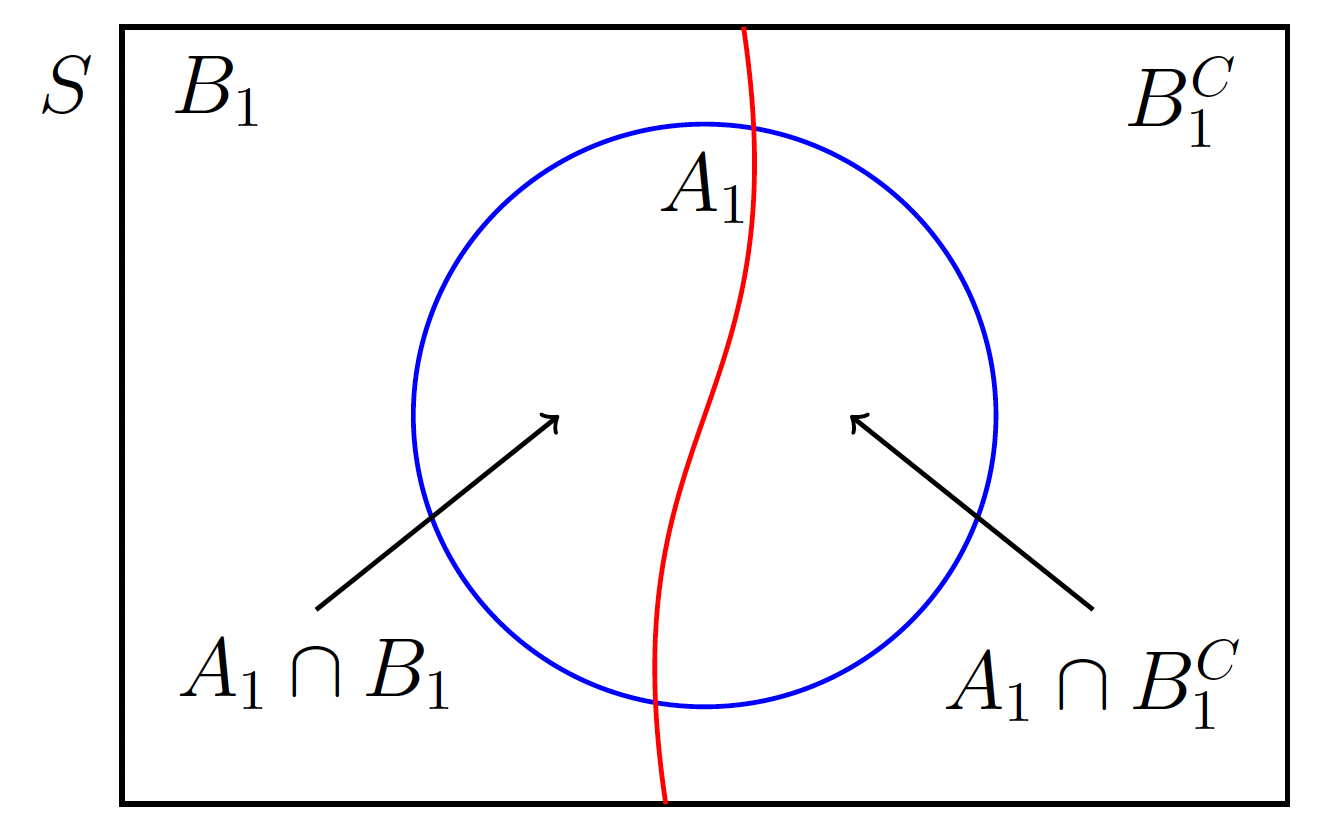
\includegraphics[width=8cm]{marginal.png}
\end{frame}
\end{document}